%/* vim: set filetype=latex */

% Demo project. Uses Komascript >=3.0. 
% which is not included in texlive 2008
% (1) copy dist to texlive/texmf-local 
% (2) texhash
%\documentclass[BCOR=8.5mm,DIV=calc,open=right,pagesize=auto,a5paper]{scrbook}
%\documentclass[12pt,BCOR=8.5mm]{scrbook}
\documentclass[12pt,BCOR=8.5mm]{scrartcl}
\title{Power to the People}
\subtitle{Bürgerorienterte Lösungen für das Stromnetz der Zukunft}
\author{Mathias Dalheimer}
%% PDF SETUP
\usepackage[pdftex, bookmarks, colorlinks, breaklinks,
pdftitle=\title,pdfauthor=\author,plainpages=false]{hyperref}  
\hypersetup{linkcolor=blue,citecolor=blue,filecolor=black,urlcolor=blue,plainpages=false} 

\clubpenalty=3000 % adjust for widows and orphans 10000 is max
\widowpenalty=3000 % adjust for widows and orphans 10000 is max
%% Font Adjustments
%\usepackage[LY1]{fontenc}
\usepackage[T1]{fontenc}
%\usepackage{adobegaramond}
%\usepackage{gillsans}
%\renewcommand{\rmdefault}{HoeflerText}

% Use URW Garamond No. 8 as a default font. (getnonfreefonts)
\usepackage[urw-garamond]{mathdesign}
%\renewcommand{\rmdefault}{ugm}
% Optima as a sans serif font.
\renewcommand*\sfdefault{uop}

\newcommand*\imgwidth{0.8\textwidth}

\usepackage{ifthen}
\newboolean{InternalVersion}
\setboolean{InternalVersion}{true}
%\setboolean{InternalVersion}{false}

\usepackage{listings}  
\lstset{numbers=left, numberstyle=\tiny,numbersep=5pt}  
\lstset{language=Xml, basicstyle=\small, frame=shadowbox}  

\usepackage{algorithmic}
\usepackage{algorithm}
%\numberwithin{algorithm}{chapter} 
%\newcommand{\theHalgorithm}{\arabic{algorithm}}

\usepackage[protrusion=true,expansion=true]{microtype}

%% Page Header
\usepackage{scrpage2}

% Recalculate page setup based on new font.
\KOMAoptions{DIV=last}
%\KOMAoptions{draft=true}

% Versals. 
%\usepackage{lettrine}
% Misc packages
\usepackage{url}
\usepackage{graphicx}
\usepackage{todonotes}
%\usepackage[english]{babel}
\usepackage{ngerman}
% Use utf-8 encoding for foreign characters
\usepackage[utf8]{inputenc}
\usepackage{blindtext}
\usepackage{subfigure}

\hyphenation{scho-oner Sur-vivor ap-pen-dix}

%% Chapterstyle
%\renewcommand*{\chapterformat}{---\hskip.5cm\thechapter\hskip.5cm---}
%\KOMAoption{headings}{small,twolinechapter}
%\setkomafont{chapter}{\Large\sffamily\centering}
%\setkomafont{dictum}{\normalfont}
%\renewcommand*{\dictumwidth}{.8\textwidth}

%% Main.
\begin{document}
\maketitle
\clearscrheadfoot
\automark[chapter]{section}
\lehead[]{\pagemark\hskip.5cm\vrule\hskip.5cm\title}
\rohead[]{\headmark\hskip.5cm\vrule\hskip.5cm\pagemark} 
\title
%\pagestyle{scrplain}
%\begin{titlepage}
%%/* vim: set filetype=tex */

%\vspace*{\baselineskip} 
\vfill 
\hbox{% 
\hspace*{0.2\textwidth}% 
\rule{1pt}{\textheight} 
\hspace*{0.05\textwidth}% 
\parbox[b]{0.75\textwidth}{ 
\vbox{% 
%\vspace{0.1\textheight} 
{\noindent\huge\sffamily \title\\[0.5\baselineskip] }
\\[2\baselineskip] 
{\Large\sffamily \subtitle}\\[4\baselineskip] 
{\Large\sffamily \author }
\\[\baselineskip] 
{\Large\sffamily dalheimer@itwm.fhg.de}\par
\vspace{0.5\textheight} 
{\noindent Auf dem Weg zum Energiesystem für die nächsten 50 Jahre}\\[\baselineskip] 
}% end of vbox 
}% end of parbox 
}% end of hbox 
\vfill 
%\null 

%\end{titlepage}
%% frontmatter
%%\input{frontmatter}
%%\parindent.0cm
%%\parskip.4cm
%%\input{pagetwo}
\parindent.4cm
\parskip.0cm
\pagestyle{scrheadings}

\section{Einleitung}
Wenn morgens in Deutschland die Kaffeemaschinen angeschaltet werden,
sorgt ein komplexes System dafür, dass der Tag gut anfängt: Unser
Stromnetz. Das deutsche Stromnetz ist über die vergangenen 100 Jahre
gewachsen und transportiert den Strom von Kraftwerken zu den
Verbrauchern. Bildlich kann man sich das anhand des "`Stromsees"' vor
Augen führen:

\begin{figure}[htbp]
  \begin{center}
    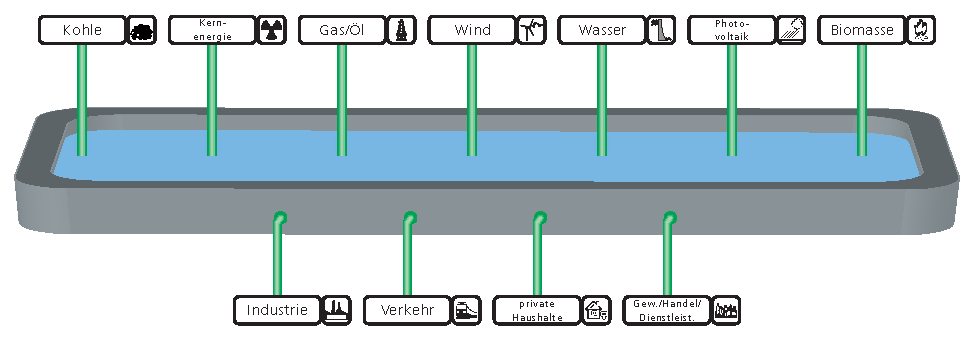
\includegraphics[width=12cm]{figures/stromsee}
    \caption{Der Stromsee: Kraftwerke erzeugen Strom, der in den
    gemeinsamen Stromsee engespeisst wird. Alle Verbraucher beziehen 
    ihren Strom aus diesem Netz.}
    \label{fig:figures/stromsee}
  \end{center}
\end{figure}


Die einzelnen Kraftwerke produzieren aus verschiedenen Energiequellen
elektrischen Strom. Der Strom wird im Netz gesammelt, bis ein beliebiger
Verbraucher den Strom benötigt\footnote{Streng genommen wird Strom
natürlich nicht verbraucht, ich bleibe allerdings bei dieser
umgangssprachlichen Formulierung.}. Konventionelle Kohlekraftwerke
tragen genauso wie Atomkraftwerke und Photovoltaiksysteme zur
Stromerzeugung bei. Das Stromnetz wird mit einem Wasserleitungssystem
verglichen.  So anschaulich dieses Modell ist, so vereinfacht es
leider zu stark:

\begin{enumerate}
  \item Der Stromsee suggeriert, dass der "`Wasserstand"' im See steigen
    und fallen kann. Das ist im Stromnetz nicht möglich, es gibt keinen
    Speicher, der Abweichungen zwischen Erzeugung und Verbrauch
    kompensieren könnte:
    \begin{equation}
      \textrm{Erzeugung}(t) = \textrm{Verbrauch}(t) + \epsilon \hspace{2cm} \forall t
    \end{equation}
    Die Erzeugung muss zu jedem Zeitpunkt dem Verbrauch entsprechen ---
    kleinere Abweichungen führen zur Änderung der Netzfrequenz, größere
    Abweichungen können zu großflächigen Stromausfällen führen. Es
    ist die Aufgabe der Stromnetzbetreiber, einen zuverlässigen Betrieb sicherzustellen. Dazu
    wird die Stromerzeugung permanent dem Verbrauch
    angepasst~\cite{wikipedia10kraftwerksmanagement}. Es
    ist nicht möglich, beliebige Kapazitäten bei Bedarf an- und
    abzuschalten: Die Anfahrvorgänge von Kraftwerken dauern je nach
    Kraftwerkstyp zwischen wenigen Minuten (Wasserkraft- und
    Gasturbinenkraftwerke) und mehreren Stunden (Kohlekraftwerke). Umgekehrt
    ist es auch nicht ohne weiteres möglich, die Leistung innerhalb von
    kurzer Zeit beliebig zu reduzieren. 

    \begin{figure}[htbp]
      \begin{center}
        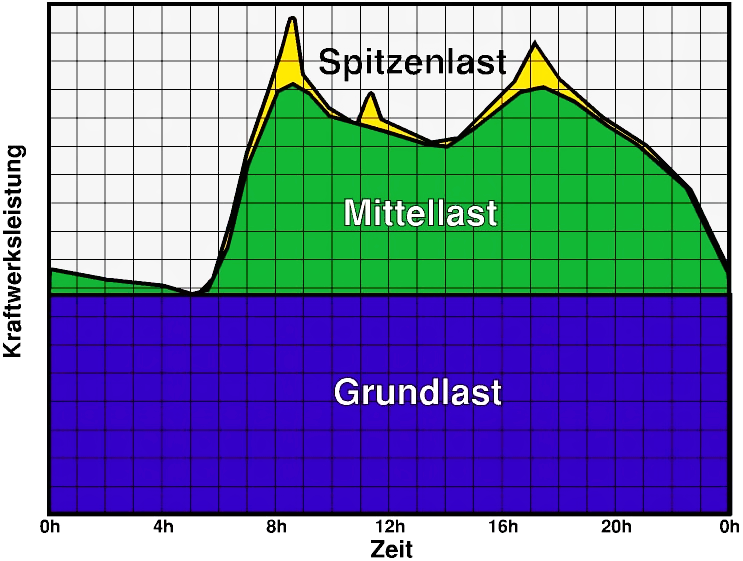
\includegraphics[width=12cm]{figures/Stromnetz_Lastkurve.png}
        \caption{Lastkurve. Quelle: \url{http://de.wikipedia.org/w/index.php?title=Datei:Stromnetz_Lastkurve.png}}
        \label{fig:stromnetz_lastkurve}
      \end{center}
    \end{figure}
    
    Die Netzbetreiber müssen also die Schwankungen des Stromverbrauchs
    vorhersagen und auch kurzfristig auf Änderungen reagieren. Dabei
    unterscheidet man zwischen Grund-, Mittel- und Spitzenlast, vlg.
    Abbildung~\ref{fig:stromnetz_lastkurve}: Die
    Grundlast ist der Bedarf, der über 24 Stunden hinweg konstant
    bleibt, quasi der Grundverbrauch. Dieser wird üblicherweise durch
    Grundlastkraftwerke wie Braunkohle- und Atomkraftwerke erzeugt. Auch
    Laufwasserkraftwerke werden üblicherweise zu den
    Grundlastkraftwerken gerechnet. Die Regelfähigkeit dieser Kraftwerke
    spielt eine untergeordnete Rolle, die Stromstückkosten stehen im
    Vordergrund: Die Erzeugung einer Kilowattstunde ist in diesen
    Kraftwerken am billigsten. Daher werden diese Kraftwerke wenn
    möglich rund um die Uhr unter Volllast betrieben.

    Die Mittellast entspricht den grundlegenden Schwankungen im
    Tagesablauf: Nachts wird erheblich weniger Energie verbraucht als
    tagsüber. Die Mittellast ist relativ gut planbar und
    wird daher z.B. mittels Steinkohlekraftwerken abgedeckt. Die
    Spitzenlast ist zwar auch planbar, aber mit erheblich mehr
    Unsicherheit verbunden. Diese Spitzenlast muss kurzfristig durch das
    Zuschalten von Spitzenlastkraftwerken wie Gasturbinenkraftwerken,
    Pumpspeicherkraftwerken oder Druckluftspeicherkraftwerke abgedeckt
    werden. Spitzenlastkraftwerke können ihre Leistung zum Teil bis zu
    20\% ihrer Nennleistung innerhalb einer Minute
    ändern~\cite{wikipedia10spitzenlast}. Da Spitzenlastkraftwerke
    nur selten unter Volllast betrieben werden, ist der erzeugte Strom
    relativ teuer: Je nach Versorgungslage kann eine Kilowattstunde
    $\euro 1,50$ kosten~\cite{wikipedia10regelleistung}. 

    Nicht in die aktive Netzregelung einbezogen sind Industriebetriebe
    mit eigener Stromerzeugung, Windkraftanlagen, Photovoltaiksysteme
    und auch Blockheizkraftwerke. 

    Für die Regelung hat das "`European Network of Transmission System
    Operators for Electricity"' (ENTSO-E) Standards geschaffen. Im
    "`UCTE Operation Handbook"' sind die Verfahren der Netzregelung im
    Abschnitt "`Load Frequency Control and Performance"'
    beschrieben~\cite{entsoe10ucte}. Als Regelgröße dient die
    Netzfrequenz: Dieser Wert muss bei 50 Hz liegen. Wenn ein
    elektrischer Verbraucher eingeschaltet wird, dann sinkt die
    Netzfrequenz. Wird umgekehrt ein Verbraucher ausgeschaltet, so
    steigt die Netzfrequenz. Genau umgekehrt wird die Netzfrequenz von
    der Leistung der Kraftwerke beeinflusst: Wird zusätzliche Leistung
    eingespeisst, so steigt die Netzfrequenz.

    Drei verschiedene Stufen sind an der Regelung beteiligt:
    \begin{enumerate}
      \item Für die \emph{Primärregelung} müssen Netzbetreiber innerhalb
        von 30 Sekunden zwei Prozent seiner aktuellen Erzeugung als
        Reserve bereitstellen bzw. die Erzeugung reduzieren können. Die
        Kraftwerke müssen bis zu 15 Minuten diese Leistungserhöhung
        liefern können. Die Primärregelung hat die Aufgabe, die
        Netzfrequenz im Höchstspannungsnetz auf europäischer Ebene
        stabil zu halten.
      \item Die \emph{Sekundärregelung} kann zeitgleich zur
        Primärregelung anlaufen und hat die Aufgabe, die
        Frequenzstabilität im einer Regelzone sicherzustellen. Dazu
        werden zusätzliche Spitzenlastkraftwerke benutzt. Die
        Sekundärregelung soll nach 15 Minuten abgeschlossen sein.
      \item Auch bei der \emph{Tertiärregelung} oder auch
        \emph{Minutenreserve} ist das Ziel, die Netzfrequenz zu
        stabilisieren. Hierbei werden zusätzliche Reserven vom
        Übertragungsnetzbetreiber bei den Lieferanten angefordert. Dies
        geschieht üblicherweise telefonisch. Die veränderte
        Lastsituation wird dann permanent durch die Kraftwerke
        abgedeckt, die Regelung ist abgeschlossen.
    \end{enumerate}

  \item Der Stromsee vernachlässigt auch, dass die Erzeugung und der
    Verbrauch von Strom geographisch verteilt sind. Eine Kilowattstunde
    aus einem Grundlastkraftwerk wird normalerweise in das
    Höchstspannungsnetz (220 und 380 Kilovolt) eingespeist, vgl. Tabelle
    \ref{tab:stromkreise}. Die Aufgabe des Höchstspannungsnetzes ist die
    Verteilung des Stroms über größere Distanzen, auch in das
    europäische Ausland. Nahe den Verbrauchszentren wird der Strom in
    das Hochspannungsnetz transformiert, von dort aus auch in das
    Mittelspannungsnetz. Mittelgroße Kraftwerke speisen in das
    Hochspannungsnetz ein, während Stadtwerke und große Windkraft- bzw.
    Photovoltaikanlagen auch direkt in das Mittelspannungsnetz
    einspeisen können. 

    \begin{table}
    \centering
    \begin{tabular}{|l|r|r|}
      \hline
      & Installierte Länge (km) & Spannung (kV) \\
      \hline
      Höchstspannung & 36.000 & 220 und 380 \\
      Hochspannung & 75.200 & 60-220 \\
      Mittelspannung & 493.000 & 6-60 \\
      Niederspannung & 1.067.100 & 0,4\\
      \hline
    \end{tabular}
    \caption{Stromkreise in Deutschland. Quelle: BMWi~\cite{bmwi10stromnetze}}
    \label{tab:stromkreise}
  \end{table}
 
    Über Umspannwerke in den Gemeinden wird das Mittelspannungsnetz an
    das Niederspannungsnetz angeschlossen. Hier wird der Strom
    schließlich durch private Haushalte und Gewerbebetriebe verbraucht.
    Eine Ausnahme stellen Industrieabnehmer dar: Diese können ihren
    Strom auch aus dem Mittelspannungsnetz beziehen.

    Die Einspeisung von Solaranlagen auf den Dächern der Privathaushalte
    kann zu Problemen bei der Netzregulierung führen: Da auf der
    Nierderspannungsebene keine Regelenergie zur Verfügung steht, können
    signifikante Photovoltaikeinspeisungen die Netzfrequenz nach oben
    treiben. Daher kommt es schon heute --- vor allem in ländlichen
    Regionen --- vor, dass die Netzbetreiber den Anschluss von
    Photovoltaikanlagen verweigern. Darüber hinaus kann eine Einspeisung
    von dezentral erzeugtem Solarstrom auch die Leitungen als solche
    überlasten.
   
  \item Der Stromsee stellt schließlich auch die Organisationsstruktur
    des Stromnetzes nicht dar. Hier sind zunächst die vier großen
    Übertragungsnetzbetreiber Amprion (RWE/VEW), EnBW Transportnetze AG,
    Transpower Stromübertragungs GmbH (TenneT) sowie 50Hertz
    Transmission (Vattenfall) zu nennen, vgl. Abbildung \ref{fig:regelzonen}.
    \begin{figure}[htbp]
      \begin{center}
        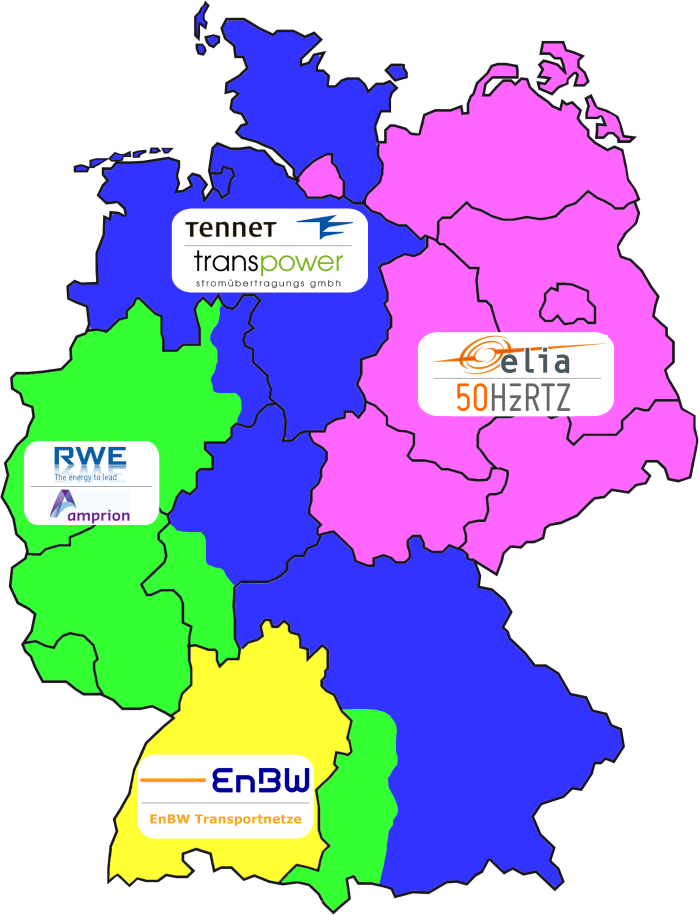
\includegraphics[width=12cm]{figures/Regelzonen_deutscher_Netzbetreiber_neu.png}
        \caption{Überblick über die Regelzonen im deutschen Stromnetz.
        CC-BY-SA Ice gixxe}
        \label{fig:regelzonen}
      \end{center}
    \end{figure}
%http://de.wikipedia.org/w/index.php?title=Datei:Regelzonen_deutscher_%C3%9Cbertragungsnetzbetreiber_neu.png&filetimestamp=20100621164106
    Die vier großen Übertragungsnetzbetreiber sind am ENTSO-E
    beteiligt und damit auch an der aktiven Netzregelung. Sie betreiben
    die Höchst- und Hochspannungsnetze. Hinzu kommen
    noch ca. 900 Verteilnetzbetreiber in Deutschland, welche die Mittel-
    und Niederspannungsnetze betreiben. Diese agieren
    lokal und stellen die Versorgung der Haushalte in ihrem
    Versorgungsgebiet sicher. Oft sind diese Verteilnetzbetreiber in der
    Hand von Stadtwerken.

    Alle Netzbetreiber kaufen --- direkt oder indirekt --- ihren Strom
    auf zwei Märkten ein: Der Termin- und der Spotmarkt an der European
    Energy Exchange (EEX) in Leipzig. Auf dem Terminmarkt werden
    längerfristige Lieferkontrakte gehandelt. Der Spotmarkt dient
    hingegen dem An- und Verkauf von Strommengen für den folgenden oder
    auch laufenden Tag. Hier können kurzfristig Strommengen ge- und
    verkauft werden, um nicht auf kostspielige Regelenergie
    zurückgreifen zu müssen.

    Die Erzeugung des Stroms wird in Deutschland von den vier Konzernen
    Vattenfall, RWE, e-on und EnBW dominiert. Daneben gibt es eine
    große Anzahl von Stadtwerken, die mit eigenen Kraftwerken Strom
    erzeugen. Hinzu kommt noch eine Vielzahl von kleinen Erzeugern, die
    mittels BHKW und Photovoltaik lokal Strom in das Netz einspeisen.
    \todo{Bericht der Monopolkommision, Wettbewerb, Vergleich der
    Strommengen}
\end{enumerate}

Unser Stromnetz ist also weit komplexer als der Stromsee sugeriert.  Der
Ausbau der erneuerbaren Energien verändert dabei viele der
Grundannahmen, unter denen unser Stromnetz gebaut wurde. Da der
Netzbetreiber die Einspeisungen von Solaranlagen entgegennehmen und
vergüten muss, sind sowohl technische Änderungen als auch
organisatorische Anpassungen nötig.

Die Stromerzeugung aus Wind, Photovoltaik und Biomasse hat einen
steigenden Anteil, im Jahr 2009 betrug er
15,6\%~\cite{web:bmwi-energiedaten}.  Die Tendenz ist weiter steigend,
einzelne Studien gehen von einem Anteil zwischen mindestens 20
\%~\cite{dena05netzstudie1} und 47~\% ~\cite{iwes09simulation} der
Erneuerbaren Energien bis 2020 aus.  Grundsätzlich macht dieser Trend
aus ökologischer Sicht Sinn.  Die unregelmässige Verfügbarkeit des
EE-Stromes führt dazu, dass z.B. in Phasen starken Windes
Grundlastkraftwerke heruntergefahren werden müssen, um die zusätzlichen
Strommengen aufzunehmen. Die Machbarkeit ist hier umstritten:
Gegner der erneuerbaren Energien weisen darauf hin, dass
Grundlastkraftwerke nicht ohne weiteres innerhalb von Stunden
heruntergefahren werden können.  Befürworter halten dagegen, dass
aufgrund von speziellen Windprognosen die Stromeinspeisungen auf
Tagesfrist recht genau vorhergesagt werden können und daher eine
Abschaltung von Kohle- und Atomkraftwerken machbar ist.

Klar ist in jedem Fall, dass sich durch den zunehmenden Anteil
regenerativer Energien im deutschen Strommix Grundlastkraftwerke immer
schlechter auslasten lassen.  Es verändert sich auch die finanzielle
Grundlage für den Betrieb von Grundlastkraftwerken: Diese sind darauf
optimiert, möglichst permanent mit hoher Auslastung Strom zu
produzieren. 

Das derzeit praktizierte Anhalten von Windkraftanlagen in Phasen starken
Windes durch die Netzbetreiber ist aus ökologischer Sicht nicht
wünschenswert. Die Gründe hierfür liegen laut der Bundesregierung zum
einen an Verzögerungen im Netzausbau und andererseits im Fehlen von
Energiespeichern~\cite{bundesreg2010kleineanfrage}. Der Anteil des nicht
eingespeisten regenerativen Stroms wird derzeit nicht erfasst. Dies ist
umso bedauerlicher, als dass die Netzbetreiber als auch Betreiber von
Grundlastkraftwerken sind und so ein Zielkonflikt entsteht.

Zusammenfassend lässt sich festhalten: Erneuerbare Energien --- so
wünschenswert ihr Einsatz ist --- führen zu Veränderungen im Stromnetz.
Neben technischen Anpassungen sind auch ökonomische Anpassungen
notwendig. Wohin also mit dem "`grünen"' Strom? Wie kann unser Stromnetz
angepasst werden?

\section{Flexibel durch Demand-Side Management}\label{sec:demand-side_management}

Klar ist, dass unser Stromnetz flexibler werden muss. Prinzipiell gibt
es zwei Möglichkeiten, dies zu schaffen: Einerseits können
Speichermöglichkeiten für Strom im Netz geschaffen werden. In
Pumpspeicherkraftwerken kann Strom zwischengespeichert werden, in dem
Wasser von einem niedrigen Reservoir in ein höhergelegenes gepumpt wird.
Wird der Strom wieder benötigt, so wird die in der Höhe gespeicherte
Energie über ein Wasserkraftwerk wieder in Strom verwandelt.
Üblicherweise werden Pumpspeicherkraftwerke so dimensioniert, dass sie
über 4-8 Stunden ihre Leistung abgeben können. Dabei steht die Leistung
innerhalb von Minuten zur Verfügung und kann in weiten Bereichen
geregelt werden. Der Wirkungsgrad liegt
bei ca. 80\%~\cite{wikipedia10pumpspeicher}.

Eine zweite Möglichkeit zur Stromspeicherung liegt in modernen
Batteriespeichern. Es gibt derzeit erste Projekte, die den
großtechnischen Einsatz von Lithion-Ionen-Batterien
erproben~\cite{braun09lithium}. Dabei werden dezentral Batteriespeicher
installiert, die im Falle eines Überschusses Strom aufnehmen und später
wieder abgeben können. In die gleiche Kategorie fallen auch
Elektrofahrzeuge, die ihre Batteriekapazität nach aussen hin zugänglich
machen. Technisch sind stationäre Systeme jedoch einfacher zu betreiben:
Die Lade- und Entladeregelung muss nicht die hohen Leistungen zur
Verfügung stellen, die in einem Elektroauto notwendig sind. Darüber
hinaus werden stationäre Systeme auch nur bis zu 30\% ihrer Kapazität
entladen. Mit aktuell verfügbaren Technologien können so
Batterielebenszeiten von 25 Jahren erreicht werden. Dezentrale
Batteriespeicher haben auch den Vorteil, dass sie direkt am
Niederspannungsnetz hängen uns so z.B. die Einspeisungen von privaten
Photovoltaiksystemen aufnehmen können. Der so zwischengespeicherte Strom
belastet die Übertragungsnetze nicht, sondern verbleibt lokal in einem
Versorgungsnetz, bis der Strom dort benötigt wird.

Die zweite Möglichkeit, das Stromnetz flexibler zu machen, liegt im \emph{Demand-Side
Management}. Statt auf der Seite der Stromerzeugung und -verteilung
Änderungen vorzunehmen, wird der Verbrauch von Strom beeinflusst. Damit
ist jedoch zunächst nicht die Reduzierung des Stromverbrauchs gemeint,
obwohl dies natürlich eine sinnvolle Anstrengung ist. Stattdessen wird
der Stromverbrauch auf der Zeitachse verschoben. Das Ziel ist es,
Stromverbraucher dann zu betreiben, wenn sowieso viel Strom erzeugt
wird. Umgekehrt laufen diese Verbraucher nicht, wenn zu einem anderen
Zeitpunkt weniger Strom erzeugt wird.

Im Industriebereich ist diese Herangehensweise schon lange Standard ---
unter dem Stichwort "`Lastabwurf"' hat ein Netzbetreiber die
Möglichkeit, den Stromverbrauch von einzelnen Industriebetrieben gezielt
zu reduzieren, um Engpässe zu vermeiden. Im Gegenzug erhält der
Industriebetrieb bessere Strompreise. Ein Verteilnetzbetreiber ist so in der
Lage, relativ schnell erhebliche Lasten im Netz der momentanen Erzeugung
anzupassen. Üblicherweise sind --- unter anderen --- die folgenden Eingriffe möglich
\cite[S. 23f]{wiechmann08lastmanagement}~\cite[S. 85ff]{bmwi06eenergy}:

\begin{enumerate}
  \item \emph{Lastspitzenreduzierung:} Dabei werden einzelne Lastspitzen
    gekappt, in dem zur Spitzenzeit Verbraucher abgeschaltet werden. In
    den Spitzenzeiten werden so höhere Kosten zur Stromerzeugung
    vermieden.
  \item \emph{Lasttalauffüllung:} Falls Strom zu Grenzkosten angeboten
    werden kann, lohnt es sich, Verbraucher zu diesem Zeitpunkt zu
    betreiben. Ein Beispiel hierfür ist das Aufladen von
    Nachtspeicherheizungen, da nachts die Last im Netz gering ist.
  \item \emph{Lastverschiebung:} Generell können natürlich Lasten im
    Stromnetz auf einen anderen Zeitpunkt verschoben werden, um
    vielfältige Ziele zu erreichen. Speziell bei kurzfristigen
    Lastveränderungen ("`Flexible Load Shaping"') wird kurzfristig
    Regelenergie durch einen Lastabwurf frei.
\end{enumerate}

Allen Eingriffen gemein ist, Lastspitzen zu glätten oder zu verschieben,
um den Einsatz teurer Spitzenlastkraftwerke zu verhindern. Bei
entsprechenden Prognosen können diese Techniken auch dazu eingesetzt
werden, Strom aus den erneuerbaren Energiequellen aufzunehmen und
gezielt zu nutzen. Im Jahr 2007 nutzen die europäischen
Übertragungsnetzbetreiber Demand Side Management-Kapazitäten im Bereich von
mehreren GWh~\cite{etso07demand}. Torriti et al.~\cite{torriti10demand}
gehen von einem stetigen Wachstum der Kapazitäten in Europa aus, vgl.
Tabelle \ref{tab:drforecast}. Zusammengenommen können momentan 2,9\% der
Spitzenlast durch Demand Side Management verschoben werden.

\begin{table}
  \centering
  \begin{tabular}{|l|r|}
    \hline
    Jahr & Kapazität in GW \\
    \hline
    2008 & 11,45\\
    2010 & 11,50\\
    2013 & 12,15 \\
    2015 & 12,82 \\
    2020 & 13,32 \\
    \hline
  \end{tabular}
  \caption{Prognose der Demand Side Management-Kapazitäten im Bereich
  der UCTE. Angaben in GW}
  \label{tab:drforecast}
\end{table}

Im Privathaushalt ist Demand Side Management jedoch noch nicht im
Einsatz, hier können noch erhebliche Kapazitäten erschlossen werden. Die
Gründe hierfür sind vielfältig: 

\begin{enumerate}
  \item Die notwendige Regelungstechnik ist in nur wenigen Haushalten
    vorhanden. Die Grundlage für die Steuerung von Geräten ist ein
    Hausbus, über den Steuersignale kommuniziert werden. Die gegenwärtig
    verfügbaren Systeme (KNX, EIB) sind recht aufwendig und teuer,
    sodass hier noch weitere Entwicklungen notwendig sind.
  \item In die Haushaltsgeräte ist normalerweise kein Zugang für ein
    Energiemanagementsystem eingebaut. Zum Beispiel gibt es bei einer
    Spülmaschine üblicherweise keine Schnittstelle, um ein Startkommando
    zu übermitteln.
  \item Es gibt kaum finanzielle Anreize für Privathaushalte, um in
    diese Technologien zu investieren. Gegenwärtig sind einzig
    Nachtstromtarife darauf zugeschnitten, den Verbrauch in Nebenzeiten
    zu fördern.
\end{enumerate}


Im Rahmen der E-Energy Initiative der Bundesregierung arbeiten diverse
Projekte daran, Demand Side Management-Technologien in Haushalte zu
integrieren~\cite{web:e-energy}. Auch Gerätehersteller wie Miele
integrieren spezielle Energiemanagementschnittstellen in ihre
Geräte~\cite{miele10ifapresse}. Allen diesen Lösungen gemein ist jedoch,
dass sie modellhaften Charakter haben und allenfals in Pilotprojekten
getestet werden.

In diesen Pilotprojekten ist neben den Managementtechnologien vor allem
die Einführung von intelligenten Stromzählern (Smart Metern) ein Thema.
Smart Meter sind elektronische Stromzähler, welche die bekannten
schwarzen Ferraris-Zähler ersetzen. Sie bieten neben der Anzeige des
Gesamtzählerstandes auch die Möglichkeit, den Momentanverbrauch oder den
Wochenverbrauch anzuzeigen. Einige Modelle bieten zudem auch die
Möglichkeit, den Stromverbrauch an den Netzbetreiber zurückzumelden, oft
in 15-minütigen Intervallen. Stromkunden können, wenn
Informationen zum Momentanverbrauch unmittelbar zur Verfügung stehen,
ihr Verhalten direkt verändern und so ihren Strombezug um 15-20\%
reduzieren~\cite{geller2010smartgrid}. Ebenso ist es denkbar, mit den
gesammelten Strombezugsinformationen weiterführende Analysen
durchzuführen. Diese können zum Beispiel Verbraucher identifizieren, die
einen erheblichen Anteil am Stromverbrauch haben. Daraufhin können
automatisiert Hinweise gegeben werden, dass sich z.B. die Anschaffung
eines energiesparenden Kühlschranks schon nach einem Jahr amortisiert
hätte.

Für die Netzbetreiber bzw. den Messtellenbetreiber ist dies eine
Herausforderung, da Kunden nicht bereit sind, für die neue Messtechnik
zu bezahlen. Zwar sind durch die direkte Rückmeldung von
Stromverbrauchsdaten Einsparungen zu erwarten,
jedoch stehen diese Einsparpotentiale in keinem Verhältnis zu
den Mehrkosten der Smart Meter. Zudem erlauben gerade zeitlich eng
aufgelöste Daten im 15-Minuten-Bereich erhebliche Rückschlüsse auf die
Lebensgewohnheiten der Anschlussinhaber.


\section{Datenschutz}\label{sub:datenschutz}
Einerseits sind diese Daten natürlich für den Stromkunden interessant,
da er den Einfluss seines Verhaltens auf den Stromverbrauch vor Augen
geführt bekommt und so insgesamt weniger verbrauchen wird.

Andererseits sind die Stromverbrauchsdaten aus Netzbetreibersicht auch
sehr interessant, da sich hier völlig neue Möglichkeiten für
Preismodelle und auch für das Marketing ergeben. Dazu muss man wissen,
dass Privathaushalte im Moment durch Standardlastprofile abgerechnet
werden, d.h. ein Verteilnetzbetreiber wird nicht für die real gelieferte
Strommenge bezahlt, sondern auf der Basis eines durchschnittlichen
Lastprofils und der Anzahl der versorgten Haushalte wird eine Pauschale
abgerechnet. Mit Smart Metern kann nun der reale Verbrauch bestimmt
werden und wird in Zukunft wohl zur Grundlage der Abrechnung werden
\footnote{Entsprechende Änderungen werden derzeit von der
Bundesnetzagentur diskutiert.}. 

Um diese Abrechnung vorzunehmen gehen die Netzbetreiber davon aus, dass
die Stromverbrauchsdaten in hoher zeitlicher Auflösung an sie übertragen
werden, um dann eine verbrauchsgenaue Abrechnung gegenüber den
Stromanbietern machen zu können. Diese Daten sind jedoch als sehr
sensibel einzustufen, da hieraus auf Lebens- und Konsumgewohnheiten
geschlossen werden kann. 

Ein beispielhafter Tagesverlauf des Autors ist in Abbildung
\ref{fig:schlaflos} dargestellt.
\begin{figure}[htbp]
  \begin{center}
    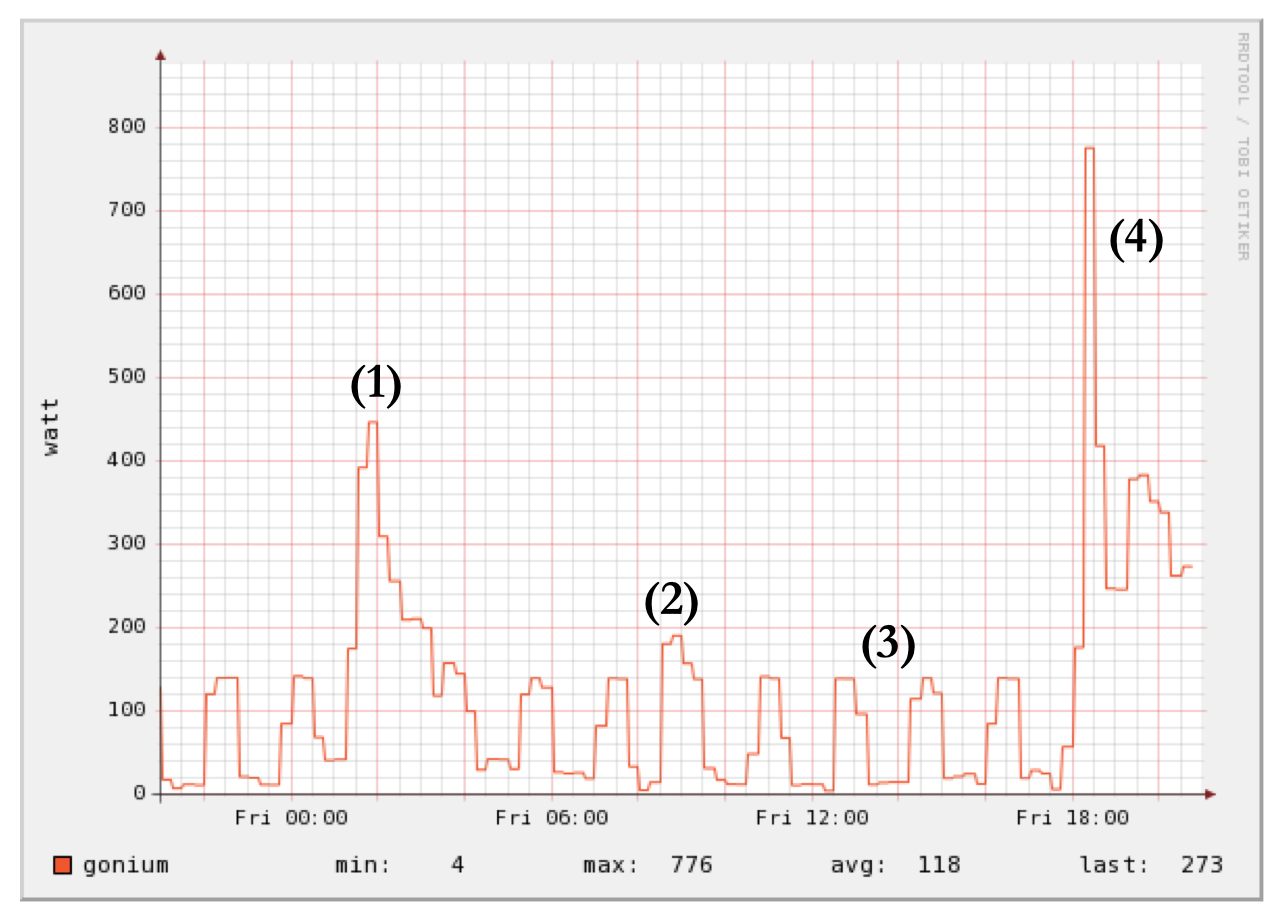
\includegraphics[width=12cm]{figures/lastkurve-md-annotated.png}
    \caption{Der Stromverbrauch des Autors am Beispiel eines Tages.}
    \label{fig:schlaflos}
  \end{center}
\end{figure}
Die Kurve gibt den Stromverbrauch in einem fünfminütigen Intervall
wieder. Bei Markierung (1) ist der Autor aufgestanden, weil er aufgrund
einer Kanada-Reise an Jetlag litt. Die Benutzung von Wasserkocher und
der Rechners schlägt sich deutlich nieder. Gegen 4:00 wurde
weitergeschlafen. Um acht Uhr morgens (2) läuft die kleine
Senseo-Kaffeemaschine, tagsüber war der Autor arbeiten. Während dieser
Zeit führt der Kühlschrank zu regelmässigen Ausschlägen (3). Gegen 18:00
kam der Autor nach Hause und benutzte die Mikrowelle.

Die Gerätesignaturen sind natürlich spezifisch für einzelne Geräte bzw.
Betriebszustände. Eine Waschmaschine bietet verschiedene Programme, die
auch zu leicht unterschiedlichen Signaturen führen. Zusätzlich führt die
Reduktion auf --- in diesem Beispiel --- fünf-Minuten-Messintervalle zum
Verlust von Information. Die Senseo-Kaffeemaschine (2) zeigt bei
einminütigen Messintervallen einen recht spezifischen Spitzenverbrauch
von 1400 Watt für ca. 1 Minute. Wenn die Werte jedoch als
Durchschnittsverbrauch der letzten fünf Minuten dargestellt werden,
bleibt davon nur noch eine kleine Spitze übrig.

Derzeit sehen die Smart Meter-Infrastrukturen eine zeitnahe Übermittlung
von 15-Minuten-Intervallwerten an die Messstellenbetreiber vor. Daraus
lassen sich immer noch einzelne Geräte identifizieren, wobei natürlich
wenig charakteristische Signaturen herausgemittelt
werden\footnote{Auch hier gilt natürlich das Nyquist-Theorem.}. Dennoch
ergeben sich hier erhebliche Privacy-Probleme: Durch statistische
Verfahren lässt sich recht einfach entscheiden, wie oft und wie lange
ein Bewohner in der Wohnung ist. Daraus kann zum Beispiel abgeleitet
werden, ob der Bewohner einer regelmässigen Tätigkeit nachgeht. Weitere
Betrachtungen zu dieser Thematik finden sich bei \todo{Referenz Artikel
KJM, FAZ-Artikel Constanze Kurz}

Derzeit argumentieren die Messstellenbetreiber, dass die Installation
von Zählern und die Übertragung und Speicherung von Verbrauchsdaten für
die Abrechnung notwendig ist. Die Einwilligung zur Datenverarbeitung
lassen sie sich durch den Anschlussinhaber bestätigen. Da dieser jedoch
üblicherweise gar keine andere Wahl hat, steht diese Argumentation
juristisch auf tönernen Füßen~\todo{DuD, Gutachten}. 

Auch wenn die Daten anonymisiert werden würden, lassen sich unter
Umständen die Datenbestände wieder auf einzelne Personen bzw.
Messstellen beziehen. So weisen Narayanan und Shmtikov auf die Möglichkeiten der
``De-Anonymisierung'' von Datensätzen hin~\cite{narayanan2010pii}. Sie
beschreiben dabei die prinzipielle Unmöglichkeit, einmal erhobene Daten
zu anonymisieren und dabei die Rückverfolgbarkeit auszuschliessen.
Ebenso argumentiert Shapiro und weist darauf hin, dass Privacy als
nichtfunktionale Anforderung nur als Designkriterium am Anfang in die
Systementwicklung integriert werden kann~\cite{shapiro2010privacy}. Eine
nachträgliche Integration von Privacy in ein bereits existierendes
System ist quasi nicht möglich.

Als Fazit lässt sich festhalten, dass einmal in Umlauf gebrachte Daten
wieder auf individuelle Verbraucher zurückgeführt werden können.
Stromverbrauchswerte sind in ihrer Sensibilität mit Bankdaten
gleichzusetzen sind. Es ist unverständlich, dass hier keine besonderen
Anforderungen an die Verarbeitung von solchen Daten vorgesehen sind.

Generell ist die Datenübertragung zum Messstellenbetreiber natürlich
nicht zur Abrechnung erforderlich. Moderne Zähler sind mit mehreren
"`Zählregistern"' ausgestattet. Abhängig von einzelnen Tarifstufen
werden gemessene Kilowattstunden auf den verschiedenen Zählregistern
erfasst. Einmal im Monat können diese Zählregisterstände dann an den
Messstellenbetreiber übertragen werden, ohne dass Rückschlüsse auf die
Lebensgewohnheiten des Anschlussinhabers möglich sind. Auch die
Bundesnetzagentur hat die Anforderungen an Smart Meter kürzlich
konkretisiert: Eine zeitnahe Übertragung der Messwerte an den
Messstellenbetreiber ist nicht erforderlich\todo{Referenz Stellungnahme EDL21-Zähler
Bundesnetzagentur}. In den Niederlanden wurde eine Smart
Metering-Infrastuktur flächendeckend installiert. Nach Bekanntwerden der
Datenschutz-Problematik wurde die Fernauslesung aufgrund von massiven
Protesten bis jetzt nicht in Betrieb genommen\todo{Quelle suchen}.
Bleibt zu hoffen, dass es in Deutschland nicht zu einer vergleichbaren
Situation kommt.

\section{Open-Source Demand Side Management: mySmartGrid}\label{sec:chancen_open-source}
\todo{MARK}
In kundenfreundlichen Lösungen liegt die Chance für Open-Source
Technologien. Indem die Technologien direkt von den Anwendern entwickelt
werden, sind die Chancen groß, dass der Nutzen für Privathaushalte im
Vordergrund steht.  In Zusammenarbeit mit kleinen Stadtwerken in
öffentlicher Hand kann eine Strommanagement-Infrastruktur kostendeckend
etabliert werden.

Im Projekt \emph{mySmartGrid} wird zur Zeit in Kaiserslautern eine
entsprechende Infrastruktur aufgebaut. Das Projekt wird vom Land
Rheinland-Pfalz im Rahmen des Konjunkturprogramm II gefördert. Alle
Technologien werden in enger Zusammenarbeit sowohl mit den
Stromverbrauchern als auch mit den Netzbetreibern aus der Region
(Technische Werke Kaiserslautern, Pfalzwerke) entwickelt.  Wir bauen auf
ein Ökosystem von freien Lösungen.  Bei der Hardware setzen wir auf
Consumer-Geräte, die einen hohen Verbreitungsgrad haben.  Ein möglichst
großer Anteil der Funktionen soll in Software implementiert werden, da
diese quasi ohne weitere Kosten vervielfältigt werden kann.
Selbstverständlich werden alle Projektresultate (Soft- und Hardware)
unter einer Open-Source Lizenz veröffentlicht. 

Gleichzeitig werden ca.  1000 Haushalte in Kaiserslautern und Umgebung
mit der Technik ausgerüstet. Da die Installation von Geräten durch
Handwerker aus der Region erfolgt, ist eine möglichst gute
Installationsunterstützung durch Softwarewerkzeuge notwendig.

Das Projekt ist in drei Phasen gegliedert, die ich im Folgenden
darstelle.

\subsection{Messen und Verstehen}\label{sub:messenverstehen}

In der ersten Projektphase geht es darum, den Teilnehmern ein
Verständnis für den individuellen Stromverbrauch zu geben. Hierzu
benutzen wir den "`Flukso"', um den den Stromverbrauch eines Haushalts
zentral zu messen.\todo{Bild Flukso einfügen, Link}. Technisch ist der
Flukso ein WLAN-Router, basiert auf OpenWRT und benutzt einen kleinen
Mikrocontroller zur Messwerterfassung. Die Installation erfordert keine
Neuverkabelung, da die Messung indirekt über Halleffektsensoren erfolgt.
Die Messwerte werden zur mySmartGrid-Webseite übertragen, wo sie
visualisiert werden können. Ausserdem können die Messwerte auch lokal
abgefragt werden.

Die Daten werden auf der mySmartGrid-Webseite nicht dauerhaft
gespeichert, sondern nach und nach vergessen. Für die erste Stunde sind
Minutenwerte gespeichert, für die letzten 24 Stunden nur noch
fünfminütige Werte. Danach sinkt die Auflösung rapide. Wer die Daten
dennoch in hoher Auflösung haben möchte, muss die API der Webseite
benutzen. Weil viele Teilnehmer dies tun möchten, haben wir auch einen
"`Rekorder-Dienst"' implementiert, welcher die Daten in höchster
Auflösung mitschreiben kann. 

Es sind auch Open-Source Alternativen zum Flukso vorhanden, zum Beispiel
der Volkszähler \todo{link}. Obwohl wir ihn in diesem Projekt nicht einsetzen, sind
im Moment Diskussionen im Gange, die Schnittstellen des Fluksos und des
Volkszählers kompatibel zu machen. Aber auch die kommerziellen und von
den Netzbetreibern eingesetzten Smart Meter müssen eine lokal
auslesbare, optische Schnittstelle bieten \todo{Quelle: Positionspapier
Bundesnetzagentur}.  Die Umsetzung dieser Schnittstelle bleibt jedoch
zunächst dem Hersteller überlassen. Viele Hersteller setzen auf den
elektronischen Einheitszähler, der vom VDE \todo{Referenz
Netzkompetenzzentrum} standardisiert wird. Über die optische serielle
Schnittstelle wird jede Sekunde ein Datagramm mit allen relevanten
Informationen ausgesandt. Ein Mikrocontroller mit zugehöriger Fotodiode
ist prinzipiell alles, was zum Auslesen benötigt wird --- eine
Open-Source Lösung hierfür fehlt jedoch derzeit.

Das Messen ist allerdings zumeist nicht genug, um eine nachhaltige
Änderung des Stromverbrauchsverhaltens anzuregen. Dazu setzen wir auf
zwei Ansätze:

\begin{enumerate}
  \item Einerseits helfen automatisierte Analysen, den eigenen
    Stromverbrauch zu beurteilen. Dazu sind zunächst recht fein
    aufgelöste Stromverbrauchswerte nötig, um einzelne Verbraucher
    erkennen zu können. Daher muss dieses Verfahren optional bleiben und
    nur bei Bedarf vorgenommen werden. Wir schneiden dann für zwei
    Wochen die Stromverbrauchswerte mit und identifizieren einzelne
    Verbraucher. Basierend auf dieser Analyse ist es dann recht einfach,
    konkrete Handlungsempfehlungen zu geben, z.B. "`Tauschen Sie Ihren
    Kühlschrank aus --- das amortisiert sich nach $2,4$ Jahren."' 
    Diese Analysen sind im Moment noch im Forschungsstadium.
  \item Andererseits ist es für Stromkunden hilfreich, den Effekt ihrer
    Handlungen unmittelbar zu sehen. Wenn ich den Wasserkocher
    einschalte, dann verbrauche ich auf einmal 2kW - das führt zu einem
    gut sichtbaren Sprung in der Stromverbrauchskurve. Die logische
    Konsequenz wäre es, nur die wirklich benötigte Menge Wasser in den
    Wasserkocher zu füllen.
\end{enumerate}

Zur Anzeige der Verbrauchsinformationen haben wir uns für den
"`Chumby"` entschieden\todo{Bild}. Der Chumby basiert technisch
ebenfalls auf einem WLAN-Router, hat allerdings einen Touchscreen und
einen Lautsprecher integriert. Es sind schon viele Applikationen für den
Chumby verfügbar, sodass das Gerät neben Stromverbrauchsinformationen
auch den Wetterbericht anzeigen und Internetradio abspielen kann. Unsere
Nutzer können sich die Applikationen selbst zusammenstellen. Welche
Darstellungsformen für die Strominformationen am Sinnvollsten sind,
werden wir in der kommenden Zeit zusammen mit unseren Projektteilnehmern
erarbeiten.

\todo{Andere Anwendung, z.B. Monitoring von PV-Anlagen und Assisted
Living}

\subsection{Regelung von Verbrauchern}\label{sub:steuern}

Der nächste Schritt ist das Steuern von Verbrauchern im Haushalt.
Mit Hilfe von meteorologischen Modellen ist es möglich, die
Stromproduktion auf Tagesfrist recht genau vorherzusagen. Wenn also
morgen Mittag der Wind weht, führt dies auch zu einer erhöhten
Stromproduktion. Diese Information kann dann einen Tag im Voraus zu den
Haushalten transportiert werden. Die Nutzer können dann diese
Information angezeigt bekommen und ihr Verhalten entsprechend anpassen
--- für eine Spülmaschine ist es meist recht egal, ob sie morgens oder
mittags läuft.

Natürlich ist dies aber nicht genug, denn eigentlich sollte diese
Regelung automatisch passieren. Leider bieten die meisten
Haushaltsgeräte keine Möglichkeit, Steuerbefehle à la "`heute mittag um
14:00 Strom verbrauchen"' zu verarbeiten. \footnote{Meines Wissens nach
gibt es nur eine Waschmaschine von Miele, die es überhaupt erlaubt, in
ein Hausbussystem integriert zu werden.} Ebenso ungelöst ist die Frage
nach einem universellen und nachrüstbaren Bussystem, welches diese
Steuerinformationen zu den Verbrauchern transportiert. Bussysteme wie
EIB und KNX sind nur dann sinnvoll einsetzbar, wenn gleichzeitig größere
Umbauten an der Wohnung vorgenommen werden. Darüber hinaus sind diese
Systeme auch recht teuer. Dies schließt alle Leute aus, die in einer
Mietwohnung wohnen, denn beim Auszug ist es nicht ohne weiteres
möglich, das Bussystem mitzunehmen.

Mit "`digitalStrom"' wird derzeit ein anderes System entwickelt, welches
mit relativ geringem Aufwand nachrüstbar ist und Steuerinformationen
über das Stromnetz transportiert. Dieses System ist jedoch noch nicht am
Markt verfügbar.


Langfristig ist eine Lösung wünschenswert, die eine IP-basierte
Kommunikationsinfrastruktur auf kleinen Mikrocontrollern umsetzt, damit
die Lösung bezahlbar bleibt. Meine eigenen Experimente mit 6LoWPAN und
funkbasierter Kommunikation auf der Basis von 868 MHz zeigen, dass eine
solche Lösung sehr wohl kostengünstig umzusetzen ist\todo{Referenz
Octobus, Bild}. Mit Contiki \todo{Referenz} steht auch ein Open-Source
Betriebssystem zur Verfügung. Alternativ ist auch mit Ethersex
\todo{Referenz} eine etablierte Lösung vorhanden. 

Um die Entwicklung voran zu treiben setzen wir im Projekt mySmartGrid
auf die Steuerung von Wärmespeichern wie Kühlgeräte und Wärmepumpen. Wir
greifen dabei nicht in die interne Regelung der Geräte
ein\footnote{Es wäre für unsere Teilnehmer wohl nicht akzeptabel, wenn
ich mit meinem Lötkolben an ihren Kühlschränken herumbastele ;-)}. Für
Kühlschränke und Gefriertruhen bevorzugen wir folgenden Ansatz: Die
Geräte werden über einen Zwischenstecker von der Stromversorgung
getrennt. In der Folge steigt die Innentemperatur an. Wenn nun der
Stromverbrauch zu einem Zeitpunkt $t$ maximiert werden soll, muss die
Innentemperatur zu diesem Zeitpunkt also recht hoch sein. Dann wird das
Kühlgerät wieder ans Netz angeschlossen. Die Regelung des Kühlgerätes
wird nun aufgrund der (relativ) hohen Innentemperatur den Kompressor
anschalten und wie gewünscht Strom verbrauchen. Diese Herangehensweise
darf jedoch nicht dazu führen, dass Lebensmittel verderben oder
Tiefkühlware auftaut.

Eine einfache Lösung wäre, die Innenraumtemperatur des Kühlgerätes über
einen Sensor zu überwachen. Dieser Sensor verursacht jedoch
Zusatzkosten. Daher prognostizieren wir das Verhalten der internen
Regelung des Gerätes und übersteuern diese gezielt. Das setzt eine
Systemidentifikation und eine Einrichtungsprozedur voraus. Diese
ermittelt dann Regelparameter, die dazu benutzt werden, das Kühlgerät
gezielt vor dem geplanten Anschaltzeitpunkt auszuschalten. Gleichzeitig
ist gewährleistet, dass die Kühlkette nicht unterbrochen wird. Aus den
Strommessungen lässt sich lokal auch feststellen, ob der Kompressor
eines Kühlgerätes anläuft. Durch kurzes Einschalten ist es auch ohne
Temperatursensor möglich, Rückschlüsse auf die Innentemperatur des
Kühlgerätes zu ziehen.


Der wichtigste Faktor ist jedoch die Akzeptanz der Technologie bei den
Anwendern: Diese müssen jederzeit in der Lage sein, die vorgeschlagenen
Regeleingriffe abzulehnen. Da die Regelungsalgorithmen sowieso auf dem
Chumby laufen werden, ist hier auch der logische Platz, um den Benutzer
über die aktuelle Planung zu informieren. Dort wird es dann auch die
Möglichkeit geben, die Regelung zu beeinflussen oder auch zu
deaktivieren.

Schliesslich ist eine weitere Gruppe von Stromkunden sehr interessant
für den Einsatz von Haussteuerungen: Für Photovoltaikanlagenbesitzer ist ab
diesem Sommer der Eigenverbrauch des selbst erzeugten Stroms die
rentabelste Option\todo{Kleines Rechenbeispiel}.

Die Hersteller von Wechselrichtern für Solaranlagen sind dabei,
entsprechende Managementfunktionen in ihre Geräte zu integriern. Dabei
rechnen sie damit, dass zwischen 30 und 50 \% des eigenen Solarstroms
selbst verbraucht werden können\cite{ossenbrinck10herstellung}.

TODO: Lösung von Conergy kostet 850-900 Euro. Rentabilität? Nur für
diesen einen Zweck einsetzbar?

Ausserdem: Connergy will 2011 auch Energiespeicher für Zuhause anbieten
(Li-Ion, 8kWh). Lebensdauer > 20 Jahre.

IBC Solar: 700 Euro, Amortisation nach 5-7 Jahre bei einer 5kWp-Anlage.

Als Geräte favorisieren sie Tiefkühlanlagen.

Dies macht auch
ökonomisch Sinn, denn der selbstverbrauchte Strom muss nicht über das
Stromnetz transportiert werden und entlastet es. Ein teurer Netzausbau
kann so vielleicht nicht ganz vermieden, aber doch verzögert bzw.
reduziert werden.

Hier ist es wiederum möglich, die Stromproduktion für den folgenden Tag
recht genau vorherzusagen. Neben der Anzeige auf dem Chumby können auch
Geräte so gesteuert werden, dass sie den selbst produzierten Solarstrom
direkt aufnehmen.

\subsection{Virtueller Verbraucher}\label{sub:virtuellerverbraucher}
Natürlich ist es für einen einzelnen Haushalt nicht möglich,
signifikanten Einfluss auf das Stromnetz zu haben. Allerdings gibt es ja
recht viele Haushalte, auf die man potentiell Einfluss nehmen könnte.
Alle Teilnehmer rufen also einen Tag im Voraus die Prognose für den
nächsten Tag ab und versuchen, diese umzusetzen. Die genaue Modellierung
ist hier ein statistisches Problem, denn nicht jeder Haushalt wird sich
an die Handlungsempfehlungen halten. Zusammengenommen dürfte es jedoch
möglich sein, einen signifikanten Einfluss auf das lokale Stromnetz zu
haben.

Dieser Eingriff bietet Chancen für die lokalen Netzbetreiber. Diese
können dieses Regelpotential in ihre kurzfristige Planung mit
einbeziehen. Wenn normalerweise Lastspitzen durch den teuren,
kurzfristigen Zukauf von Strom abgedeckt werden müssen, können sie durch
die Verschiebung von Lasten Geld sparen. Diesen Profit können sie sich
dann mit den teilnehmenden Haushalten teilen. Hier sind zwei Modelle denkbar: 
\begin{enumerate}
  \item Die Haushalte schliessen sich zu einer Genossenschaft zusammen
    und verhandeln direkt mit dem lokalen Netzbetreiber. Die Vermarktung
    des Regelpotentials ist nicht an einen Stromlieferanten gebunden,
    d.h. die Eigner der Genossenschaft können ihren Strom bei
    unterschiedlichen Lieferanten einkaufen. Die Einnahmen der
    Genossenschaft können zur Finanzierung der Geräte verwendet werden.
    Dieses Modell macht dort Sinn, wo kleinere Netzbetreiber wie
    unabhängige Stadtwerke den Netzbetrieb organisieren.
  \item Ein anderes Modell wäre die Finanzierung der Geräte etc. über
    den Stromvertrieb, d.h. ein Stromkunde bekommt andere
    Lieferkonditionen, wenn er mit der Regelung seiner Geräte
    einverstanden ist. Hier hat der Stromkunde gegenüber dem
    Genossenschaftsmodell eine schwächere Position. Zudem ist dieses
    Modell aufgrund der Organisation des Strommarkts schwierig
    umzusetzen.
\end{enumerate}

Für mySmartGrid favorisieren wir das Genossenschaftsmodell. Unser Plan
ist es, die Geräte aus dem Projekt bei den Teilnehmern zu belassen und
die Gründung einer Genossenschaft anzustoßen. Die Herausforderung
bleibt: Wie kann Demand-Side Management kostendeckend eingesetzt werden?


Gleichzeitig sind hier natürlich Probleme des Systemdesigns zu beachten:
Als großes verteiltes System muss die Umsetzung zu einem stabilen
Systemverhalten führen. Ausfälle von einzelnen Systemkomponenten dürfen
nicht zu Störungen des Gesamtsystems führen.

Wir favorisieren dabei einen dezentralen Ansatz: Steuergeräte in den
einzelnen Haushalten verhalten sich dabei autonom. Lediglich ein
gewünschtes Lastprofil wird den Haushalten vorgegeben. Die einzelnen
Haushalte entscheiden dann autonom, wie einzelne Geräte zu steuern sind.
Die Verteilung des Lastprofils kann dabei durch standardisierte
Protokolle über das Internet erfolgen.


Kunden müssen diesen Mehrwert sehen und bereit sein, in diese Technik zu
investieren. Dies kann natürlich auch komplett an den Stromversorgern
vorbei passieren, siehe oben: Wenn die mySmartGrid-Technologie
installiert ist, kann eine Genossenschaft gegründet werden.

TODO: Modellierung von verschiedenen Lastgängen durch die Kombination
von Schaltzeitpunkten und Gruppen von Haushalten / Gewerbebetrieben.
Eventuell dynamische Anpassung der Gruppen, um gleiche ``Steuergrößen''
pro Gruppe abrufen zu können. 



\section{Schlussfolgerungen}
Smart Grids, "`intelligente Stromnetze"', sind eines der Themen, welche
von der Politik und natürlich auch der Stromwirtschaft immer wieder in
den Vordergrund gestellt werden. Leider kommt dabei der Stromkunde zu
kurz --- die Bedürfnisse von Stromkunden werden weitgehend ignoriert und
der Datenschutz wird oft ausser acht gelassen\todo{Referenz
BMWi-Konferenz Nutzerschutz}.

Aber auch kleinere Stadtwerke haben mit dieser Entwicklung Probleme:
Aufgrund politischer Vorgaben müssen sie zum Beispiel Smart Meter
einführen, obwohl ihnen dadurch Kosten entstehen, die sie nicht direkt
auf den Kunden umlegen können. 

Für die Netzbetreiber / Messtellenbetreiber ist dies eine
Herausforderung, da Kunden nicht bereit sind, für die neue Messtechnik
zu bezahlen. Daher müssen Mehrwerte geschaffen werden.

Kunden müssen diesen Mehrwert sehen und bereit sein, in diese Technik zu
investieren. Dies kann natürlich auch komplett an den Stromversorgern
vorbei passieren, siehe oben: Wenn die mySmartGrid-Technologie
installiert ist, kann eine Genossenschaft gegründet werden.

Gleichzeitig ist die Einführung von "`intelligenten"' Technologien in
das Stromnetz eine hervorragende Spielwiese für alle Hacker und Nerds.
Hier gilt es, Gedanken umzusetzen, die sowieso in den Hackerspaces
dieser Welt diskutiert werden\footnote{Warum definiert jeder Hackerspace
ein eigenes Hausbussystem?}. Das Problem rein technologisch anzugehen
wäre allerdings zuwenig. Sowohl ökonomische, ökologische als auch
gesellschaftliche Überlegungen müssen mit einbezogen werden. Es wird
auch immer mehr als eine Lösung geben. Insofern sind die idealen
Voraussetzungen für ein Open-Source Ökosystem gegeben --- lasst uns diese
Spielwiese nutzen!

\cite{geller2010smartgrid}


%%/* vim: set filetype=tex */

\section{Einleitung}\label{sec:einleitung}

Regenerative Energien, Zuwachs in Zukunft
Studie BEE als Argument benutzen

Aber: Problem Produktion und Verbrauch von elektrischer Energie.
Grundannahme: Entnahme = Einspeisung zu jedem Zeitpunkt

\begin{enumerate}
  \item Grundlastkraftwerke: Vor allem Braun- und Steinkohlekraftwerke,
	aber auch Atomkraftwerke.
  \item Volatile Kraftwerke: Wind und Sonne, aber auch Gaskraftwerke.
	Unterscheidung in planbare und nicht planbare Erzeugung von
	Elektrizität.
\end{enumerate}

Erneuerbare-Energien-Gesetz: Der Netzbetreiber muss die Einspeisungen
von Solaranlagen entgegennehmen und vergüten. Das hat Folgen für
die Netzstabilität.

Business von Netzbetreibern: Stabilität des Netzes sicherstellen. Dabei
vom Vertrieb getrennt. Stromeinkauf einerseits langfristig (OTC),
andererseits kurzfristiger Zukauf von Ausgleichsenergie.

Vgl. auch Einleitung DuD (KJM)

TODO: Mit Bichler reden, um die Fakten richtig hinzubekommen.

Zentrale Frage: Wie kann man als Netzbetreiber mit volatiler Stromeinspeisung umgehen?
Traditioneller Weg: Zur Erzeugung von Ausgleichsstrom werden auch
Gaskraftwerke hoch- bzw. heruntergeregelt. Diese Kapazitäten werden in
Zukunf allerdings nicht ausreichen.

Im Prinzip zwei Möglichkeiten:
\begin{enumerate}
  \item Speicherung von Strom, z.B. in Pumpspeicherkraftwerken oder
	Batterien. Problem: Die Kapazitäten reichen nicht aus. 
  \item Demand-Side Management: Verlagerung von Lasten auf der
	Zeitachse.
\end{enumerate}

Schließlich führt die Erhebung von Stromverbrauchsinformationen auch zur
Veränderung von Konsumgewohnheiten. Stromkunden können, wenn
Informationen zum Momentanverbrauch unmittelbar zur Verfügung stehen,
ihr Verhalten direkt verändern und so ihren Strombezug um 15-20\%
reduzieren~\cite{geller2010smartgrid}. Ebenso ist es denkbar, mit den
gesammelten Strombezugsinformationen weiterführende Analysen
durchzuführen. Diese können zum Beispiel Verbraucher identifizieren, die
einen erheblichen Anteil am Stromverbrauch haben. Daraufhin können
automatisiert Hinweise gegeben werden, dass sich z.B. die Anschaffung
eines energiesparenden Kühlschranks schon nach einem Jahr amortisiert
hätte.


TODO: Grundlegende Terminologie festlegen.
Netzbetreiber, Verbraucher (gerät), Stromkunde, Strombezug (anstatt
Stromverbrauch)

%%/* vim: setformat tex
%*/

\section{Demand Side Management}\label{sec:demandside}
Natürlich ist es erstrebenswert, absolut gesehen weniger Strom zu
verbrauchen\footnote{Die Autoren sind sich darüber im klaren, dass Energie
nicht verbraucht werden kann --- wir folgen jedoch dem allgemeinen
Sprachgebrauch.}. Allerdings ist dies nicht das Ziel des Demand-Side
Managements. Stattdessen wird hier versucht, den Verbrauch an die
Erzeugung von Strom anzupassen. Dieses Verfahren ist seit langem in der
Industrie üblich --- großen Verbrauchern aus der Industrie werden
vergünstigte Preise eingeräumt, wenn dafür im Falle von Netzengpässen
der Stromverbraucher abgeschaltet werden können. 

Dazu teilt der Netzbetreiber dem Großverbraucher auf kurze Sicht (15
Minuten) mit, dass einige Aggregate abzuschalten sind. Daraufhin werden
Spitzen im Strombedarf gekappt.

TODO: Verschiedene Szenarien, siehe eEnergy-Studie

Das gleiche Grundprinzip kann natürlich auch im Haushalt umgesetzt
werden. Hier muss es jedoch das Ziel sein, eine kostengünstige Umsetzung
ohne Komforteinbußen für den Verbraucher zu realisieren. Dazu spielt
natürlich auch der Preis eine Rolle. Zudem ist der verschiebbare
Stromverbrauch eines einzelnen Verbrauchers nicht groß im Vergleich zu
der benötigten Ausgleichsenergie. Allerdings kann durch die Kombination
einer hinreichend großen Anzahl an Haushalten ein signifikanter
Verbrauch verschoben werden. Diese Ansammlung von Haushalten und
natürlich auch Gewerbebetrieben kann als eine Einheit angesprochen
werden, wenn sie zu einem \emph{virtuellen Verbraucher}
zusammengeschlossen werden.

TODO: Kommerzielles Modell. Wie kann Demand-Side Management im
Privathaushalt nachhaltig werden? Angedacht ist der Verkauf der
Ausgleichsenergie an den Netzbetreiber. Dieser müsste nicht zu hohen
Preisen Strom kaufen bzw. verkaufen. Diese Marge kann sich der
Netzbetreiber mit den Privathaushalten teilen. Dzu gründen die
Privathaushalte eine Genossenschaft und verhandeln mit dem
Netzbetreiber. Statt eines niedrigeren Strombezugspreis (vgl. Yello
SmartMeter) kann der Preis hier freier verhandelt werden. Der Vertrieb
der Stromversorger wird umgangen.

Gleichzeitig sind hier natürlich Probleme des Systemdesigns zu beachten:
Als großes verteiltes System muss die Umsetzung zu einem stabilen
Systemverhalten führen. Ausfälle von einzelnen Systemkomponenten dürfen
nicht zu Störungen des Gesamtsystems führen.

Wir favorisieren dabei einen dezentralen Ansatz: Steuergeräte in den
einzelnen Haushalten verhalten sich dabei autonom. Lediglich ein
gewünschtes Lastprofil wird den Haushalten vorgegeben. Die einzelnen
Haushalte entscheiden dann autonom, wie einzelne Geräte zu steuern sind.
Die Verteilung des Lastprofils kann dabei durch standardisierte
Protokolle über das Internet erfolgen.

TODO: Modellierung von verschiedenen Lastgängen durch die Kombination
von Schaltzeitpunkten und Gruppen von Haushalten / Gewerbebetrieben.
Eventuell dynamische Anpassung der Gruppen, um gleiche ``Steuergrößen''
pro Gruppe abrufen zu können. 


%%/* vim: setformat tex
%*/

\section{Umsetzung}\label{sec:umsetzung}

Hier besteht die Gefahr, das Feld komplett den kommerziellen Anbietern
zu überlassen. Dies ist nicht unbedingt im Sinne der privaten
Verbraucher. Gleichzeitig werden auch kleinere Stadtwerke im Wettbewerb
übervorteilt, wenn große Stromanbieter ihre Infrastrukturen auf ihren
eigenen Gewinn hin optimieren. 

Wir gehen daher einen anderen Weg und 

%%/* vim: set filetype=tex */

\section{Risiken}\label{sec:risiken}
Die Einführung von SmartMetern birgt erhebliche Risiken für die
Privatsphäre. Definition Privacy vs. Security

Quellen: Google Powermeter, Hersteller, Erfassung von
15-Minuten-Interfaces
Stellungnahme der Bundesnetzagentur zu den §21 EnGG. Welche Kriterien
sind tatsächlich nötig?
DuD-Artikel

So weisen Narayanan und Shmtikov auf die Möglichkeiten der
``De-Anonymisierung'' von Datensätzen hin~\cite{narayanan2010pii}. Sie
beschreiben dabei die prinzipielle Unmöglichkeit, einmal erhobene Daten
zu anonymisieren und dabei die Rückverfolgbarkeit auszuschliessen.
Ebenso argumentiert Shapiro und weist darauf hin, dass Privacy als
nichtfunktionale Anforderung nur als Designkriterium am Anfang in die
Systementwicklung integriert werden kann~\cite{shapiro2010privacy}. Eine
nachträgliche Integration von Privacy in ein bereits existierendes
System ist quasi nicht möglich.

Fazit: Einmal in Umlauf gebrachte Daten können wieder auf individuelle
Verbraucher zurückgeführt werden.


\begin{enumerate}
  \item Zeige \& erkläre einen Tagesverlauf, zeige, dass daraus sehr
	persönliche Informationen extrahiert werden können.
  \item Diskutiere rechtliche Rahmenbedingungen: DuD-Artikel, Gutachten
	ULD Schleswig-Holstein -> gesetzliche Rahmenbedingungen müssen
	geschaffen werden.
\end{enumerate}

Durch die Kontrolltechnik werden DDOS-Attacken auf das Stromnetz möglich
-> Alle Verbraucher könnten zum gleichen Zeitpunkt angeschaltet werden.
Dies ist eine Herausforderung für Systemdesigner.

Für die Netzbetreiber / Messtellenbetreiber ist dies eine
Herausforderung, da Kunden nicht bereit sind, für die neue Messtechnik
zu bezahlen. Daher müssen Mehrwerte geschaffen werden.

Kunden müssen diesen Mehrwert sehen und bereit sein, in diese Technik zu
investieren. Dies kann natürlich auch komplett an den Stromversorgern
vorbei passieren, siehe oben: Wenn die mySmartGrid-Technologie
installiert ist, kann eine Genossenschaft gegründet werden.

%\section{Weitere Anwendungen}\label{sec:weitere_anwendungen}
Die Investitionen in das intelligente Stromnetz können auch eine Reihe
von weiteren Applikationen fördern, bzw. diese Applikationen
beschleunigen die Umsetzung von Smart Grid Technologien:

\begin{enumerate}
  \item Home Automation: Wenn ein Hausbussystem installiert wurde,
	können einerseits natürlich Steuerinformationen aus dem Stromnetz
	transportiert werden. Andererseits können diese Bussysteme natürlich
	auch für Komfortfunktionen etc. verwendet werden. Hier ergeben sich
	im besten Falle auch Synergien. Problematisch ist jedoch die
	fehlende Standardisierung und Nachrüstbarkeit in Mietwohnungen.
	Ebenfalls stellt sich die Frage, wie Hausbussysteme im Bestand
	kostengünstig integriert werden können.
  \item Assisted Living: Hier können Smart Meter eine interessante
	Ergänzung zu vielen integrierten Sensoren liefern. Die Zeiten
	zwischen den Aktivitäten von elektrischen Geräten geben Auskunft
	über die Aktivitäten der Bewohner.
  \item Eigenverbrauch von Photovoltaik-Strom optimieren
  \item Analyse und Überwachung von Photovoltaik-Anlagen
	(herstellerunabhängig)
\end{enumerate}




%\section{Ökosystem}\label{sec:ökosystem}
Ziel einerseits, Entwicker in die Infrastrukturentwicklung einzubinden,
andererseits auch, Verbrauchergemeinschaften zu bilden. Da alle
Komponenten als Open-Source Software und Hardware von jedem modifiziert
werden können, erwarten wir, dass viele induviduelle Anpassungen
entstehen werden.


\begin{enumerate}
  \item Viel Raum für eigene Ideen (Spieltrieb)
  \item Grundlage: Billige Vernetzung, Preise müssen weiter sinken
  \item NAchrüstbarkeit der Technologie in existierenden Wohnungen
  \item Regelungsalgorithmen bzw. Adapter für Geräte
  \item Analyse von Stromverbrauchsmustern
\end{enumerate}


\bibliographystyle{plain}
\bibliography{main}
\end{document}

% usage of todo package:
%\todo{foobar.}
%\missingfigure{A big black toad.}


